% Copyright 2011-2015 David Hadka.  All Rights Reserved.
%
% This file is part of the MOEA Framework User Manual.
%
% Permission is granted to copy, distribute and/or modify this document under
% the terms of the GNU Free Documentation License, Version 1.3 or any later
% version published by the Free Software Foundation; with the Invariant Section
% being the section entitled "Preface", no Front-Cover Texts, and no Back-Cover
% Texts.  A copy of the license is included in the section entitled "GNU Free
% Documentation License".

\chapter{Parallelization}
\label{chpt:parallelization}

When we first introduced the \java{Executor} class in \chptref{chpt:executor}, we demonstrated the \java{distributeOnAllCores()} method as a way to automatically and seamlessly distribute the evaluation across all cores in your local computer.  This section shows how to expand this simple distributed computing methods to large-scale cloud and high-performance computing systems.

We will explore three classes of parallelization: master-slave, island-model, and hybrid.  The master-slave approach will increase computing speed (decrease computing time) by spreading the function evaluations across multiple processors or computers.  The island-model approach improves convergence properties of the algorithm by running multiple concurrent instances of the MOEA, periodically sharing candidate solutions between islands (called migrations).  Lastly, the hybrid approach combines the master-slave and island-model to provide the benefits of both techniques.

\section{Master-Slave Parallelization}
\label{sect:masterSlave}

The ``master-slave'' parallelization strategy is a parallelization technique to reduce computing by spreading the workload across multiple processing cores, either on the same computer or on multiple computers connected by a network.  The MOEA is run on a single node called the master, and all function evaluations are distributed to one or more slave nodes for processing.

In order for this form of parallelization to work, the algorithm must be naturally parallelizable.  To be naturally parallelizable, the algorithm must avoid querying the evaluation results (i.e., the objectives and constraint values) prior to evaluating all solutions.  This is typically achieved by designing an algorithm to invoke the \java{evaluateAll(...)} method.  If this condition holds, then the MOEA Framework will automatically detect that the algorithm is parallelizable and enable master-slave processing.  A simple way to determine if an algorithm is parallelizable is to use the \java{distributeOnAllCores()} method in the \java{Executor} and checking the CPU usage of each core on your local computer.  Many of the algorithms provided by the MOEA Framework are parallelizable (e.g., NSGA-II, $\epsilon$-NSGA-II, NSGA-III, GDE3) but others like are not (e.g., $\epsilon$-MOEA, MOEA/D).

\begin{wrapfigure}{l}{3cm}
  
\includegraphics[width=3cm]{jppf.png}
\end{wrapfigure}
The MOEA Framework relies on third-party ``grid computing'' or ``parallel processing'' libraries to enable the distribution of work across multiple computers.  One such library is JPPF.  This section demonstrates configuring and running a master-slave MOEA using the MOEA Framework and JPPF.  This example was tested using JPPF version 4.2.5.  For the purposes of this exercise, we will run all slave nodes on a single computer.  Please refer to the JPPF documentation for information on running nodes on multiple computers.

\begin{figure}
  \center
  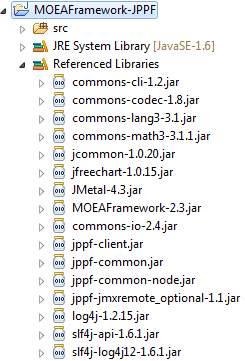
\includegraphics{jppfProjectSetup.png}
  \caption{Screenshot of an Eclipse project with the JPPF and MOEA Framework JAR files included.}
  \label{fig:jppfProjectSetup}
\end{figure}

To begin, first download the Server/Driver, Node, and Application Template distributions from \webpage{http://www.jppf.org/} and unzip the files to any location on your computer.  Next, create a new project in your Java development environment (e.g., Eclipse or NetBeans).  Add to the project the MOEA Framework and JPPF JAR files located in the \folder{MOEAFramework-%VERSION%/lib} and \folder{JPPF-4.2.5-application-template/lib} folders, respectively.  If using Eclipse, the project folder should appear similar to \figref{fig:jppfProjectSetup}. 

In this example, we will create a simple test problem and artificially make it computationally expensive by adding a long-running loop.  Create a new Java class called \file{ParallelProblem.java} with the following code:

\begin{lstlisting}[language=Java]
import java.io.Serializable;

import org.moeaframework.core.Problem;
import org.moeaframework.core.Solution;
import org.moeaframework.core.variable.EncodingUtils;

public class ParallelProblem implements Problem, Serializable {

	private static final long serialVersionUID = 5790638151819130066L;

	@Override
	public String getName() {
		return "ParallelProblem";
	}
	
	@Override
	public int getNumberOfVariables() {
		return 1;
	}

	@Override
	public int getNumberOfObjectives() {
		return 2;
	}
	
	@Override
	public int getNumberOfConstraints() {
		return 0;
	}

	@Override
	public void evaluate(Solution solution) {
		long start = System.currentTimeMillis();
		double x = EncodingUtils.getReal(solution.getVariable(0));
		
		// simulate time-consuming evaluation
		for (long i = 0; i < 500000000; i++);
		
		solution.setObjective(0, Math.pow(x, 2.0));
		solution.setObjective(1, Math.pow(x - 2.0, 2.0));
		
		System.out.println("Elapsed time: " +
				(System.currentTimeMillis() - start));
	}

	@Override
	public Solution newSolution() {
		Solution solution = new Solution(1, 2);
		solution.setVariable(0, EncodingUtils.newReal(-10.0, 10.0));
		return solution;
	}
	
	@Override
	public void close() {
		//do nothing
	}

}
\end{lstlisting}

\begin{tip}
Note that this class implements the \java{Serializable} interface.  This is a required step for parallelization.  Implementing the \java{Serializable} interface allows the Java class to be encoded and transmitted across a network.  To make a serializable class, all one needs to do is add \java{implements Serializable} after the class name, as shown in this example.
\end{tip}

Next, create another Java class called \file{JPPFExample.java} with the following code:

\begin{lstlisting}[language=Java]
import org.jppf.client.JPPFClient;
import org.jppf.client.concurrent.JPPFExecutorService;
import org.moeaframework.Executor;
import org.moeaframework.core.NondominatedPopulation;

public class JPPFExample {

	public static void main(String[] args) {
		JPPFClient jppfClient = null;
		JPPFExecutorService jppfExecutor = null;

		try {
			jppfClient = new JPPFClient();
			jppfExecutor = new JPPFExecutorService(jppfClient);
			
			// setting the batch size is important, as JPPF will only
			// run one job at a time from a client; the batch size
			// lets us group multiple evaluations (tasks) into a
			// single job
			jppfExecutor.setBatchSize(100);
			jppfExecutor.setBatchTimeout(100);
			
			long start = System.currentTimeMillis();

			NondominatedPopulation result = new Executor()
					.withProblemClass(ParallelProblem.class)
					.withAlgorithm("NSGAII")
					.withMaxEvaluations(10000)
					.distributeWith(jppfExecutor)
					.run();
			
			System.out.println("Solutions found: " + result.size());
			System.out.println("Total elapsed time: " + 
						((System.currentTimeMillis() - start) / 1000) +
						" seconds");
		} catch(Exception e) {
			e.printStackTrace();
		} finally {
			if (jppfExecutor != null) {
				jppfExecutor.shutdown();
			}

			if (jppfClient != null) {
				jppfClient.close();
			}
		}
	}
	
}
\end{lstlisting}

Line 20 is where we configure the Executor to distribute function evaluations using JPPF.  Also of importance is lines 20-21, where we set the JPPF batch size and timeout.  It is best if the batch size is equal to the population size in this example (the default population size of $100$).

With these two files created, we can now test this example.  Prior to running the Java code we just created, you will need to start the JPPF driver and one or more JPPF nodes.  To start the driver, run the \file{JPPF-4.2.5-driver/startDriver.bat} program.  To start a local node, run the \file{JPPF-4.2.5-node/startNode.bat} program.  You should see two command prompt windows appear.  If using Unix/Linux, use the files with the \plaintext{.sh} extension instead.  Once the driver and node(s) are started, run the \java{JPPFExample} class we just created.  If all works as intended, your computer should now be running at or near $100\%$ CPU utilization as it is distributing work to all nodes.

During our testing, we found that running this example on a single local core with no parallelization takes approximately $1,687$ seconds while running on four local cores takes approximately $545$ seconds.  This results in a speedup of $3.1x$.  We lose some speedup due to communication overhead between the master and slave nodes, but still obtain a reasonable speedup.

\section{Island-Model Parallelization}

Rather than run a single algorithm and distribute the problem evaluations to many cores, the island-model approach runs multiple instances of the algorithm in parallel.  This method of parallelization does not speed up the algorithm itself, but allows running multiple algorithms in parallel.  Periodically, solutions migrate from one population to another.  These migration events distribute genetic information to other islands, which in practice improves convergence properties.  For example, if one island gets stuck at a local optima, a migration event may introduce new genetic material that helps the island escape the local optima and continue searching for the global optimum.

The MOEA Framework can support island-model parallelization with some additional coding.  The developer is responsible for instantiating each algorithm/island and processing the migrations.  Below is a simple island-model example where migration events occur every $10,000$ evaluations.  A random solution from each island population is selected (the emigrant) and sent to one of the neighboring islands.  Special care is needed to ensure the code is correctly synchronized to avoid race conditions.  In this example, we use a semaphore to ensure mutual exclusion while obtaining locks (i.e., the \java{synchronized (oldIsland)} and \java{synchronized (newIsland)} lines) to avoid the possibility of deadlocks.  Additionally, the majority of Java and MOEA Framework classes are not thread safe, and any modifications must be carefully synchronized.

\begin{lstlisting}[language=Java]
import java.util.HashMap;
import java.util.Map;
import java.util.Properties;
import java.util.concurrent.Semaphore;

import org.apache.commons.math3.random.MersenneTwister;
import org.apache.commons.math3.random.RandomAdaptor;
import org.apache.commons.math3.random.SynchronizedRandomGenerator;
import org.moeaframework.algorithm.NSGAII;
import org.moeaframework.algorithm.PeriodicAction;
import org.moeaframework.algorithm.PeriodicAction.FrequencyType;
import org.moeaframework.core.NondominatedPopulation;
import org.moeaframework.core.PRNG;
import org.moeaframework.core.Population;
import org.moeaframework.core.Problem;
import org.moeaframework.core.spi.AlgorithmFactory;
import org.moeaframework.core.spi.ProblemFactory;

public class IslandExample {
	
	public static void main(String[] args) {
		final int numberOfIslands = 4;
		final int maxEvaluations = 1000000;
		final int migrationFrequency = 10000;
		final Problem problem = ProblemFactory.getInstance()
				.getProblem("DTLZ2_2");
		final Map<Thread, NSGAII> islands = new HashMap<Thread,
				NSGAII>();
		
		// this semaphore is used to synchronize locking
		// to prevent deadlocks
		final Semaphore semaphore = new Semaphore(1);
		
		// need to use a synchronized random number generator
		// instead of the default
		PRNG.setRandom(new RandomAdaptor(
				new SynchronizedRandomGenerator(
				new MersenneTwister())));
		
		// create the algorithm run on each island
		for (int i = 0; i < numberOfIslands; i++) {
			final NSGAII nsgaii = (NSGAII)AlgorithmFactory
					.getInstance().getAlgorithm(
							"NSGAII",
							new Properties(),
							problem);
			
			// create a periodic action for handling migration events
			final PeriodicAction migration = new PeriodicAction(
					nsgaii,
					migrationFrequency,
					FrequencyType.EVALUATIONS) {

				@Override
				public void doAction() {
					try {
						Thread thisThread = Thread.currentThread();
						
						for (Thread otherThread : islands.keySet()) {
							if (otherThread != thisThread) {
								semaphore.acquire();
								
								Population oldIsland = islands.get(thisThread)
										.getPopulation();
								Population newIsland = islands.get(otherThread)
										.getPopulation();
										
								synchronized (oldIsland) {
									synchronized (newIsland) {
										int emigrant = PRNG.nextInt(oldIsland.size());
										newIsland.add(oldIsland.get(emigrant));
								
										System.out.println("Sending solution " +
												emigrant + " from " +
												Thread.currentThread().getName() +
												" to " + otherThread.getName());
									}
								}
								
								semaphore.release();
							}
						}
					} catch (InterruptedException e) {
						// ignore
					}
				}
				
			};
			
			// start each algorithm its own thread so they run
			// concurrently
			Thread thread = new Thread() {
				
				public void run() {
					while (migration.getNumberOfEvaluations() <
							maxEvaluations) {
						migration.step();
					}
				}
				
			};
			
			islands.put(thread, nsgaii);
		}
		
		// start the threads
		for (Thread thread : islands.keySet()) {
			thread.start();
		}
		
		// wait for all threads to finish and aggregate the result
		NondominatedPopulation result =
				new NondominatedPopulation();
		
		for (Thread thread : islands.keySet()) {
			try {
				thread.join();
				result.addAll(islands.get(thread).getResult());
			} catch (InterruptedException e) {
				System.out.println("Thread " + thread.getId() +
						" was interrupted!");
			}
		}
		
		System.out.println("Found " + result.size() +
				" solutions!");
	}

}
\end{lstlisting}

\section{Hybrid Parallelization}

Combining the island-model and master-slave parallelization strategies, the hybrid parallelization approach inherits the benefits of both strategies.  It gains speedup from the master-slave strategy by distributing function evaluations across many cores, and the benefit of operating multiple, concurrent algorithms in the island-model strategy.  Since we are not using the \java{Executor} in the island-model example, we instead use the underlying \java{DistributedProblem} class.  To enable the hybrid strategy, wrap the problem created on lines 25-26 to either distribute work across multiple local cores:
\begin{lstlisting}[language=Java]
problem = new DistributedProblem(problem,
		Runtime.getRuntime().availableProcessors());
\end{lstlisting}
or on multiple computers across a network using JPPF:
\begin{lstlisting}[language=Java]
problem = new DistributedProblem(problem, jppfExecutor);
\end{lstlisting}

Above, \java{jppfExecutor} is the JPPF executor service created in \sectref{sect:masterSlave}.  Note that all of the requirements outlined in \sectref{sect:masterSlave} must be followed when using JPPF.

\section{Conclusion}
This chapter provided an introduction to parallel computing with the MOEA Framework.  We explored the master-slave, island-model, and hybrid parallelization strategies.  Using parallelization, we can help decrease computing time by distributing the workload across multiple computers and/or improve convergence properties by running multiple concurrent algorithms.  